\documentclass[11pt,a4paper]{article}

\usepackage[utf8]{inputenc}
\usepackage[T1]{fontenc}
\usepackage[english]{babel}
\usepackage{amsmath, amssymb, amsthm}
\usepackage{geometry}
\usepackage{hyperref}
\usepackage{booktabs}
\usepackage{array}
\usepackage{mathtools}
\usepackage{lmodern}
\usepackage{graphicx}
\usepackage{float}
\usepackage{subcaption}

\geometry{margin=2.5cm}

\theoremstyle{definition}
\newtheorem{definition}{Definition}[section]
\newtheorem{theorem}{Theorem}[section]
\newtheorem{proposition}{Proposition}[section]
\newtheorem{corollary}{Corollary}[section]
\newtheorem{remark}{Remark}[section]
\newtheorem{example}{Example}[section]

\newcommand{\cbrt}[1]{\sqrt[3]{#1}}
\newcommand{\prt}[2]{\sqrt[#1]{#2}}
\newcommand{\eps}{\varepsilon}

\title{\textbf{Generalized Pandrosion Residuals}\\[0.3em]
  \large Residual profile of an iterative geometric construction
  for $p$-th roots of any positive real number}
\author{Ivan \textsc{Besevic}}
\date{April 2026}

\begin{document}

\maketitle

\begin{abstract}
We generalize Pandrosion's geometric construction --- originally designed to approximate $\cbrt{2}$ by inserting proportional means via Thales' theorem --- to any integer $p \geq 2$ and any positive real $x$. The construction produces two sequences: an internal parameter $u_n$ and an output $v_n \to \alpha = x^{1/p}$. After normalized substitution $s_n = (C - u_n)/C$, the iteration takes the universal form involving the geometric polynomial $S_p(s) = \sum_{k=0}^{p-1} s^k$. We prove that the fixed point is $s^* = x^{-1/p} = \alpha^{-1}$, that convergence is \emph{linear}, and we compute the exact contraction ratio
\[
  \lambda_{p,x} = \frac{(\alpha - 1)\displaystyle\sum_{k=1}^{p-1} k\,\alpha^{p-1-k}}{\displaystyle\sum_{k=0}^{p-1} \alpha^k},
  \qquad \alpha = x^{1/p}.
\]
This ratio, expressed entirely in terms of the target $\alpha$, is the \emph{convergence signature} of Pandrosion's method. Closed-form expressions are given for $p=2$, $3$, and $4$. Numerical verification confirms all predictions. We compare with Newton's quadratically convergent residual profile.
\end{abstract}

\tableofcontents
\bigskip

%=====================================================================
\section{Introduction}
%=====================================================================

The Greek problem of doubling the cube consists of constructing a segment of length $\cbrt{2}$ from a unit segment. It is equivalent to finding two proportional means $m_1, m_2$ between $1$ and $2$, that is,
\[
  \frac{1}{m_1} = \frac{m_1}{m_2} = \frac{m_2}{2},
\]
which yields $m_1 = \cbrt{2}$ and $m_2 = \cbrt{4}$. Pandrosion of Alexandria proposed an \emph{approximate} geometric method, reported by Pappus in the \textit{Collectio}, Book~III~\cite{pappus}: by successive parallels (Thales' theorem), she constructs proportional ratios that approach these means without ever reaching them exactly in a finite number of steps.

\medskip

This work starts from a fundamental observation:

\begin{quote}
\itshape A real number is exact in pure mathematics. But a method to reach it possesses a measurable residual profile --- a footprint intrinsic to the method.
\end{quote}

At each finite step of Pandrosion's construction, there remains a gap $\eps_n = |v_n - \alpha|$ between the geometric approximation and the ideal value. The sequence $(\eps_n)$ is the \textbf{residual profile} of the method. Our goal is to compute this profile exactly for any $p$-th root $x^{1/p}$, and to identify the contraction ratio that characterizes Pandrosion's method.

\medskip

To our knowledge, the contraction ratio $\lambda_{p,x}$ in the form~\eqref{eq:lambda_general} does not appear in standard numerical analysis textbooks (Stoer--Bulirsch~\cite{stoer}, \textit{Numerical Recipes}~\cite{numrecipes}), nor in works devoted to the history of cube duplication. The result therefore appears to be new.

\medskip

\textbf{Outline.} Section~\ref{sec:pandrosion3} recalls Pandrosion's construction for $\cbrt{2}$ and analyzes its residual profile. Section~\ref{sec:generalisation} states the generalization to any $p, x$. Section~\ref{sec:coefficient} computes the contraction ratio $\lambda_{p,x}$ and provides closed-form expressions. Section~\ref{sec:exemples} presents numerical tables. Section~\ref{sec:comparaisons} compares with bisection, the secant method, and Newton's method. Section~\ref{sec:conclusion} concludes.

%=====================================================================
\section{Pandrosion's construction for \texorpdfstring{$\cbrt{2}$}{cbrt(2)}}
\label{sec:pandrosion3}
%=====================================================================

\subsection{The two sequences}

The geometric construction produces two sequences as a function of an initial parameter $u_0$:
\begin{equation}
  \label{eq:pandrosion_orig}
  u_{n+1} = \frac{u_n}{2 - 2\!\left(\dfrac{4 - u_n}{4}\right)^{\!3}},
  \qquad
  v_n = 2\!\left(\frac{4 - u_n}{4}\right)^{\!2},
  \qquad u_0 = 0.5.
\end{equation}

The sequence $(u_n)$ is the \emph{internal parameter} of the construction (a length in the Thales diagram). The sequence $(v_n)$ is the \emph{readout}: the approximation of $\cbrt{2}$ produced at step $n$.

\begin{proposition}
$\displaystyle\lim_{n\to\infty} v_n = \cbrt{2}$.
\end{proposition}

\subsection{Normalized substitution}

Setting $s_n = (4 - u_n)/4$, so that $s_n \in (0,1)$, we obtain:
\begin{itemize}
  \item $u_n = 4(1 - s_n)$,
  \item $v_n = 2s_n^2$,
  \item $u_{n+1} = \dfrac{4(1-s_n)}{2(1-s_n^3)} = \dfrac{2}{1 + s_n + s_n^2}$.
\end{itemize}

The iteration on $s_n$ then becomes:
\begin{equation}
  \label{eq:iter_s3}
  s_{n+1} = 1 - \frac{u_{n+1}}{4} = \frac{2s_n^2 + 2s_n + 1}{2s_n^2 + 2s_n + 2}.
\end{equation}

\subsection{Fixed point}

The fixed point $s^*$ satisfies $s^* = (2s^{*2} + 2s^* + 1)/(2s^{*2} + 2s^* + 2)$, which gives $2(1-s^*)(1+s^*+s^{*2}) = 1$, i.e.\ $2(1-s^{*3}) = 1$, hence $s^{*3} = 1/2$, so:
\[
  s^* = 2^{-1/3} = \frac{1}{\cbrt{2}}.
\]
The output at the fixed point is $v^* = 2s^{*2} = 2 \cdot 2^{-2/3} = 2^{1/3} = \cbrt{2}$. \checkmark

\subsection{Residual profile: linear convergence}

Let $h(s) = (2s^2 + 2s + 1)/(2s^2 + 2s + 2)$. The derivative at $s^*$ gives the convergence rate:
\[
  h'(s^*) = \frac{4s^* + 2}{(2s^{*2} + 2s^* + 2)^2} = \frac{2(2s^*+1)}{4(s^{*2}+s^*+1)^2} = \frac{2s^*+1}{2(s^{*2}+s^*+1)^2}.
\]

Substituting $s^* = 2^{-1/3}$ and using the closed form~\eqref{eq:lambda3}:
\[
  \lambda_{3,2} = \frac{(\cbrt{2}-1)(\cbrt{2}+2)}{\cbrt{4}+\cbrt{2}+1} \approx 0.2202.
\]

\begin{theorem}[Linear residual law for $p=3$, $x=2$]
Under the above hypotheses, for any $s_0$ sufficiently close to $s^*$:
\[
  \eps_{n+1}^{(s)} \approx \lambda_{3,2}\,\eps_n^{(s)}, \qquad \lambda_{3,2} \approx 0.2202.
\]
Since $v_n - \cbrt{2} \approx (p-1)\alpha^2\,(s_n - s^*)$ and $(p-1)\alpha^2 = 2 \cdot \cbrt{4}$, the output residual of $v_n$ converges at the same linear rate.
\end{theorem}

\begin{table}[h]
\centering
\begin{tabular}{ccccc}
\toprule
$n$ & $s_n$ & $v_n$ & $\eps_n = |v_n - \cbrt{2}|$ & $\eps_{n+1}/\eps_n$ \\
\midrule
0 & 0.8750 & 1.5312 & $2.713 \times 10^{-1}$ & --- \\
1 & 0.8107 & 1.3143 & $5.44\phantom{0} \times 10^{-2}$ & 0.200 \\
2 & 0.7974 & 1.2717 & $1.17\phantom{0} \times 10^{-2}$ & 0.216 \\
3 & 0.7945 & 1.2625 & $2.58\phantom{0} \times 10^{-3}$ & 0.219 \\
4 & 0.7939 & 1.2605 & $5.67\phantom{0} \times 10^{-4}$ & 0.220 \\
$\infty$ & $2^{-1/3}$ & $\cbrt{2}$ & $0$ & $\to \lambda_{3,2}$ \\
\bottomrule
\end{tabular}
\caption{Numerical residual profile for $p=3$, $x=2$ ($u_0 = 0.5$, i.e.\ $s_0 = 0.875$). The ratio converges to $\lambda_{3,2} \approx 0.220$.}
\end{table}

%=====================================================================
\section{Geometric origin: why $S_p$ arises naturally}
\label{sec:geometrie}
%=====================================================================

\subsection{The construction by successive parallels}

Pandrosion's construction relies on Thales' theorem applied to a rectangle. Consider a rectangle with sides $H$ and $W$ equipped with two diagonals (Figure~\ref{fig:geometry}). A horizontal line at height $u_n$ from the bottom intersects the two diagonals and defines:
\begin{itemize}
  \item the parameter $s_n = (H - u_n)/H$ (normalized position from the top),
  \item the readout length $v_n = x \cdot s_n^{p-1}$ (the output of the construction).
\end{itemize}

\begin{figure}[H]
  \centering
  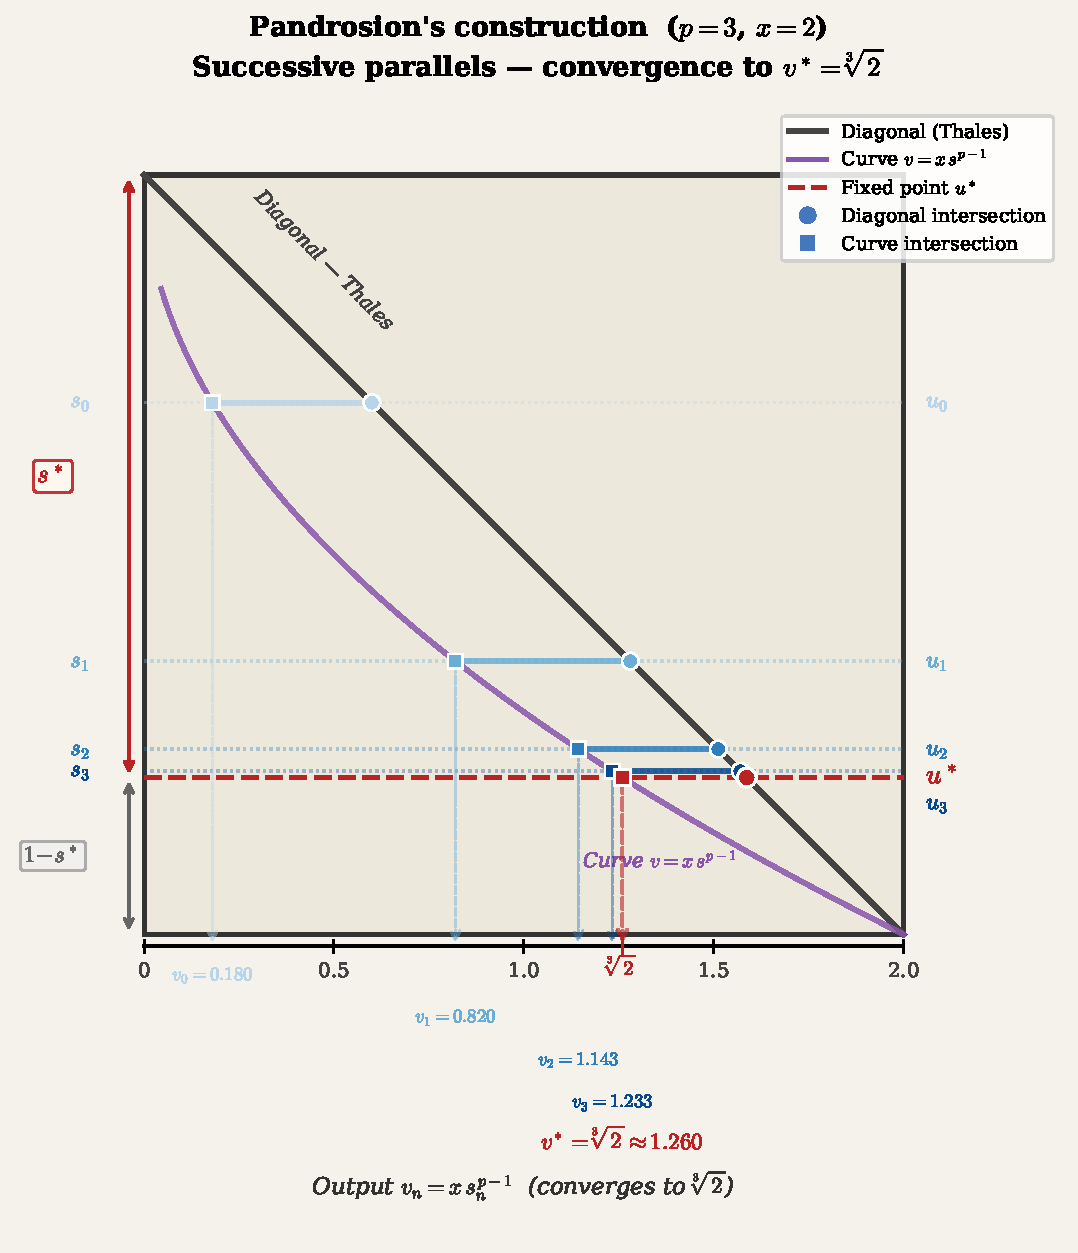
\includegraphics[width=0.52\textwidth]{pandrosion_geometry.pdf}
  \caption{Pandrosion's geometric construction for $p=3$, $x=2$.
  The blue horizontal lines (steps $n=0,1,2,3$) converge toward the dashed red line,
  which corresponds to $v^* = \sqrt[3]{2}$.}
  \label{fig:geometry}
\end{figure}

\subsection{Where does the polynomial $S_p$ come from?}

The fundamental idea is as follows. We seek to insert $p-1$ proportional means between $1$ and $x$, that is, to construct the ideal geometric sequence $1, \alpha, \alpha^2, \ldots, \alpha^{p-1}, x$ where $\alpha = x^{1/p}$. If $s_n \approx \alpha^{-1}$ is the current approximation of the inverse ratio, the sum of the approximate geometric sequence is:
\[
  S_p(s_n) = 1 + s_n + s_n^2 + \cdots + s_n^{p-1}.
\]
The ideal sequence satisfies $x \cdot S_p(s^*) \cdot (1-s^*) = x-1$, which rewrites as $x(1-s^{*p}) = x-1$. Pandrosion's correction adjusts $s_n$ so as to reduce the gap between $S_p(s_n)$ and its ideal value via the formula:
\[
  s_{n+1} = 1 - \frac{x-1}{x \cdot S_p(s_n)}.
\]
Geometrically, the ratio $(x-1)/(x \cdot S_p(s_n))$ measures the \emph{deviation} of the current proportional chain from the perfect geometric chain, and subtraction from $1$ produces the corrected ratio. The polynomial $S_p$ is thus the analytical transcription of the sum of the $p$ segments constructed via Thales' theorem.

%=====================================================================
\section{Generalization: Pandrosion's construction for \texorpdfstring{$x^{1/p}$}{x\^{}(1/p)}}
\label{sec:generalisation}
%=====================================================================

\subsection{The universal iteration}

Let $x > 0$ and $p \geq 2$ be an integer. Set $\alpha = x^{1/p}$. The generalized Pandrosion geometric construction is defined as follows.

\begin{definition}[Generalized Pandrosion iteration]
\label{def:pandrosion_gen}
We define the sequence $(s_n)_{n \geq 0}$ in $(0, 1)$ by
\begin{equation}
  \label{eq:pandrosion_gen}
  s_{n+1} = 1 - \frac{x - 1}{x \cdot S_p(s_n)},
  \qquad
  S_p(s) = \sum_{k=0}^{p-1} s^k = \frac{1 - s^p}{1 - s},
\end{equation}
and the output sequence by
\begin{equation}
  \label{eq:vn_gen}
  v_n = x \cdot s_n^{p-1}.
\end{equation}
We call $\eps_n = |v_n - \alpha|$ the \textbf{Pandrosion residual} at step $n$.
\end{definition}

\begin{remark}
For $p = 3$, $x = 2$, we recover exactly the iteration~\eqref{eq:iter_s3}. Indeed:
\[
  1 - \frac{1}{2(1+s+s^2)} = \frac{2s^2+2s+1}{2s^2+2s+2}. \checkmark
\]
\end{remark}

\subsection{Geometric interpretation}

The iteration~\eqref{eq:pandrosion_gen} analytically translates the Thales operation: at each step, $S_p(s_n)$ measures the ``geometric sum'' of the constructed segments, and the correction $(x-1)/(x \cdot S_p(s_n))$ adjusts the position proportionally to the gap with the ideal geometric sequence $1, \alpha, \alpha^2, \ldots, \alpha^{p-1}, x$.

\subsection{Fixed point}

\begin{theorem}[Fixed point]
\label{thm:fixed_point}
The unique fixed point of the iteration~\eqref{eq:pandrosion_gen} in $(0,1)$ is $s^* = x^{-1/p} = \alpha^{-1}$. The corresponding output is $v^* = x \cdot (x^{-1/p})^{p-1} = x^{1/p} = \alpha$.
\end{theorem}

\begin{proof}
At a fixed point $s^*$, we have $1 - (x-1)/(x \cdot S_p(s^*)) = s^*$, i.e.\
\[
  x \cdot S_p(s^*) \cdot (1 - s^*) = x - 1.
\]
Since $S_p(s)(1-s) = 1 - s^p$, this gives $x(1 - s^{*p}) = x - 1$, hence $s^{*p} = 1/x$, i.e.\ $s^* = x^{-1/p}$. The formula for $v^*$ follows immediately.
\end{proof}

%=====================================================================
\section{The contraction ratio \texorpdfstring{$\lambda_{p,x}$}{lambda}}
\label{sec:coefficient}
%=====================================================================

\subsection{General computation}

\begin{theorem}[Pandrosion contraction ratio]
\label{thm:lambda}
The convergence of the iteration~\eqref{eq:pandrosion_gen} toward $s^* = \alpha^{-1}$ is \emph{linear} with contraction ratio
\begin{equation}
  \label{eq:lambda_general}
  \boxed{
  \lambda_{p,x} = \frac{(\alpha - 1)\displaystyle\sum_{k=1}^{p-1} k\,\alpha^{p-1-k}}{\displaystyle\sum_{k=0}^{p-1} \alpha^k}
  }, \qquad \alpha = x^{1/p}.
\end{equation}
In particular, the residuals obey the law $\eps_{n+1} \approx \lambda_{p,x} \cdot \eps_n$.
\end{theorem}

\begin{proof}
Let $h(s) = 1 - (x-1)/(x \cdot S_p(s))$. Then
\[
  h'(s) = \frac{x-1}{x} \cdot \frac{S_p'(s)}{S_p(s)^2},
\]
where $S_p'(s) = \sum_{k=1}^{p-1} k s^{k-1}$.

At the fixed point $s^* = \alpha^{-1}$:
\begin{align*}
  S_p(s^*) &= \frac{1 - \alpha^{-p}}{1 - \alpha^{-1}} = \frac{\alpha(x-1)}{x(\alpha-1)}, \\
  S_p'(s^*) &= \sum_{k=1}^{p-1} k\,\alpha^{-(k-1)} = \alpha \sum_{k=1}^{p-1} k\,\alpha^{-k}.
\end{align*}

Substituting:
\[
  h'(s^*) = \frac{x-1}{x} \cdot \frac{\alpha \sum_{k=1}^{p-1} k\,\alpha^{-k}}{\left[\dfrac{\alpha(x-1)}{x(\alpha-1)}\right]^2}
  = \frac{x(\alpha-1)^2}{\alpha(x-1)} \sum_{k=1}^{p-1} k\,\alpha^{-k}.
\]

Multiplying numerator and denominator by $\alpha^{p-1}$, and using $x = \alpha^p$:
\[
  h'(s^*) = \frac{(\alpha-1)^2\,\alpha^{p-1}\sum_{k=1}^{p-1}k\,\alpha^{-k}}{\alpha^p - 1}
  = \frac{(\alpha-1)\sum_{k=1}^{p-1}k\,\alpha^{p-1-k}}{\sum_{k=0}^{p-1}\alpha^k},
\]
where we used $\alpha^p - 1 = (\alpha-1)\sum_{k=0}^{p-1}\alpha^k$. This establishes~\eqref{eq:lambda_general}.
\end{proof}

\begin{remark}
The contraction ratio $\lambda_{p,x}$ is entirely determined by $\alpha = x^{1/p}$: the target itself dictates the rate at which Pandrosion's method approaches it. This is the \textbf{convergence signature} of the method.
\end{remark}

\subsection{Closed forms for \texorpdfstring{$p=2$}{p=2} and \texorpdfstring{$p=3$}{p=3}}

For $p = 2$: $\sum_{k=1}^{1} k\,\alpha^{0} = 1$, $\sum_{k=0}^{1}\alpha^k = 1 + \alpha$.
\begin{equation}
  \label{eq:lambda2}
  \lambda_{2,x} = \frac{\alpha - 1}{\alpha + 1} = \frac{\sqrt{x} - 1}{\sqrt{x} + 1}.
\end{equation}

For $p = 3$: $\sum_{k=1}^{2} k\,\alpha^{2-k} = \alpha + 2$, $\sum_{k=0}^{2}\alpha^k = \alpha^2+\alpha+1$.
\begin{equation}
  \label{eq:lambda3}
  \lambda_{3,x} = \frac{(\alpha-1)(\alpha+2)}{\alpha^2 + \alpha + 1} = \frac{(\cbrt{x}-1)(\cbrt{x}+2)}{\cbrt{x^2}+\cbrt{x}+1}.
\end{equation}

For $p = 4$: $\sum_{k=1}^{3}k\,\alpha^{3-k} = \alpha^2 + 2\alpha + 3$, $\sum_{k=0}^{3}\alpha^k = \alpha^3+\alpha^2+\alpha+1$.
\begin{equation}
  \label{eq:lambda4}
  \lambda_{4,x} = \frac{(\alpha-1)(\alpha^2+2\alpha+3)}{\alpha^3+\alpha^2+\alpha+1}.
\end{equation}

\begin{remark}[Asymptotic behavior in $x$]
For fixed $p = 2$ and $x \to \infty$: $\lambda_{2,x} = (\sqrt{x}-1)/(\sqrt{x}+1) \to 1^-$. The larger $x$, the slower the convergence. For $x \to 1^+$: $\lambda_{p,x} \to 0$, convergence is very fast near $1$.
\end{remark}

\subsection{Basin of attraction}

\begin{theorem}[Global convergence]
\label{thm:bassin}
For any $x > 1$ and any $p \geq 2$, the iteration~\eqref{eq:pandrosion_gen} converges to $s^*$ for all $s_0 \in (0,1)$. Moreover, convergence is \emph{monotone}: if $s_0 < s^*$ then $(s_n)$ is strictly increasing, and if $s_0 > s^*$ then $(s_n)$ is strictly decreasing.
\end{theorem}

\begin{proof}
Set $h(s) = 1 - (x-1)/(x \cdot S_p(s))$.

\textbf{Step 1: $h$ is strictly increasing.}
We have $h'(s) = \frac{x-1}{x} \cdot \frac{S_p'(s)}{S_p(s)^2}$, where $S_p'(s) = \sum_{k=1}^{p-1} k s^{k-1} > 0$ for $s > 0$.

\textbf{Step 2: $h$ maps $(0,1)$ into itself.}
For $s \in (0,1)$: $S_p(s) > 1$ (since the first term is $1$ and the remaining terms are positive), so $h(s) = 1 - (x-1)/(x \cdot S_p(s)) < 1 - (x-1)/(x \cdot p) > 0$. More precisely, $h(0^+) = 1 - (x-1)/x = 1/x > 0$ and $h(1^-) = 1 - (x-1)/(xp) < 1$.

\textbf{Step 3: monotone convergence.}
Since $h$ is increasing and $h(s^*) = s^*$, if $s_0 < s^*$ then $s_1 = h(s_0) < h(s^*) = s^*$, and $s_1 = h(s_0) > h(0^+) = 1/x > 0$. By induction, $(s_n)$ remains in $(0, s^*)$. Moreover, $h(s) > s$ for $s < s^*$ (since $h(s) - s$ changes sign only at $s^*$ and $h'(s^*) < 1$), so $(s_n)$ is strictly increasing and bounded, hence convergent, necessarily to $s^*$. The case $s_0 > s^*$ is symmetric.
\end{proof}

\subsection{Bound on the number of iterations}

\begin{proposition}[Cost of Pandrosion's method]
\label{prop:cout}
To achieve accuracy $|v_n - \alpha| < \delta$ starting from $s_0 \in (0,1)$, the required number of iterations satisfies
\[
  n_\delta \leq \left\lceil \frac{\ln(\eps_0 / \delta)}{\ln(1/\lambda_{p,x})} \right\rceil,
\]
where $\eps_0 = |v_0 - \alpha|$ is the initial error.
\end{proposition}

\begin{proof}
Since $\eps_{n+1} \leq \lambda_{p,x}\,\eps_n$ asymptotically, we have $\eps_n \leq \lambda_{p,x}^n \eps_0$. The inequality $\lambda_{p,x}^n \eps_0 < \delta$ gives $n > \ln(\eps_0/\delta)/\ln(1/\lambda_{p,x})$.
\end{proof}

\begin{example}
For $p=3$, $x=2$ ($\lambda_{3,2} \approx 0.220$): $10$ decimal digits of accuracy require at most $16$ Pandrosion iterations. For $p=3$, $x=8$ ($\lambda_{3,8} = 4/7$): $43$ iterations are needed.
\end{example}

%=====================================================================
\section{Graphical illustrations}
\label{sec:figures}
%=====================================================================

\begin{figure}[H]
  \centering
  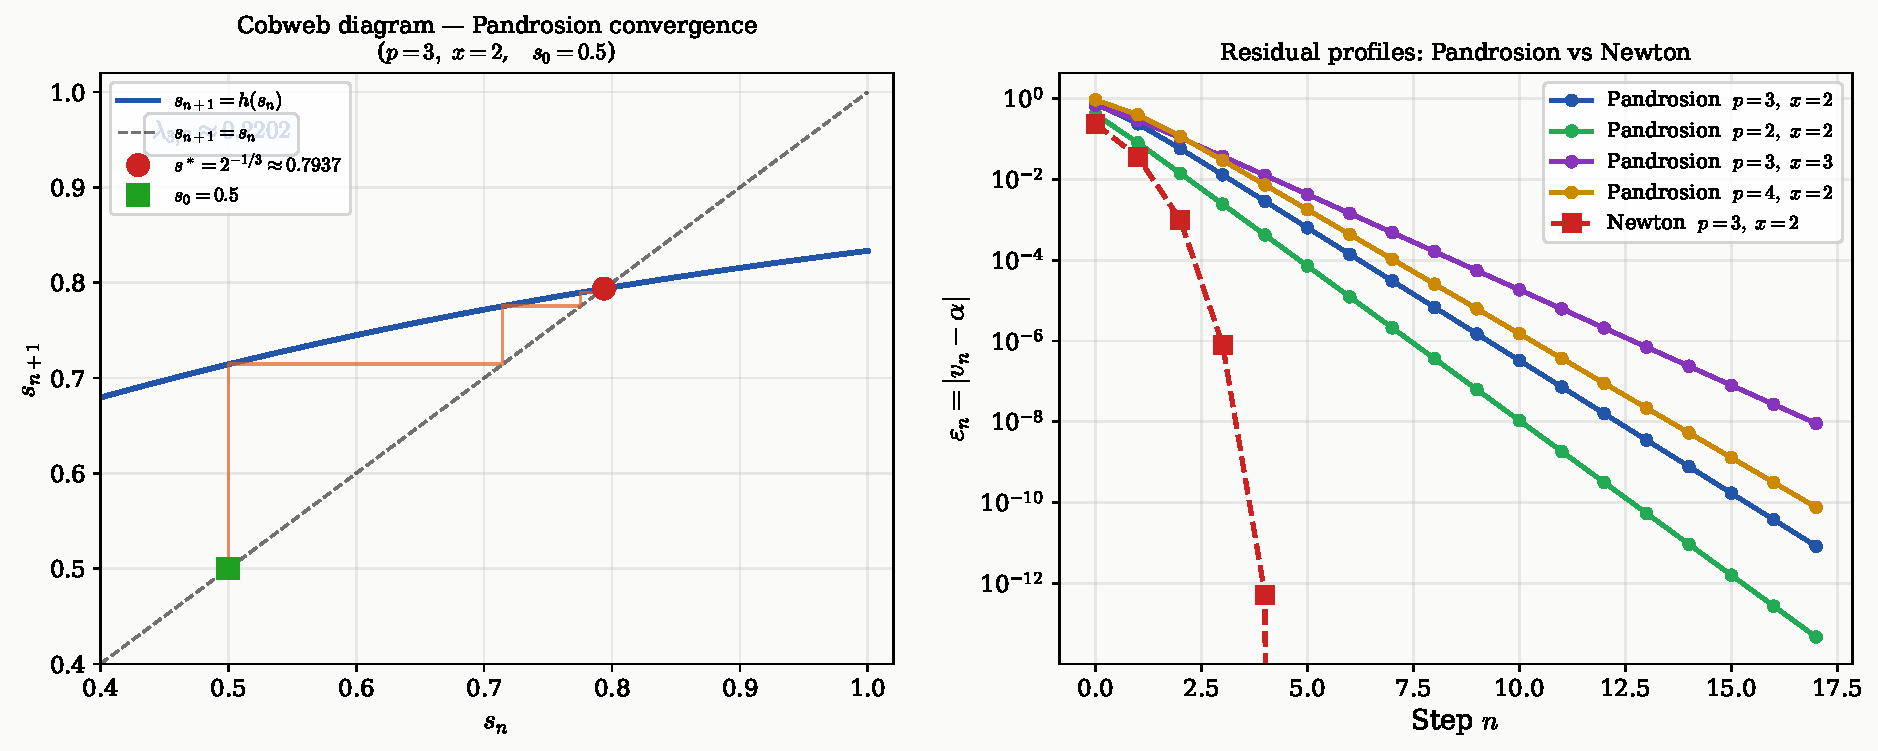
\includegraphics[width=\textwidth]{pandrosion_figures.pdf}
  \caption{\textbf{Left:} Cobweb diagram of the iteration $s_{n+1} = h(s_n)$ for
  $p=3$, $x=2$, starting at $s_0=0.875$. The spiral converges to $s^* = 2^{-1/3}$
  with rate $\lambda_{3,2} \approx 0.220$.
  \textbf{Right:} Residual profiles on a semi-logarithmic scale.
  The linear decay (straight lines) confirms the geometric convergence
  $\varepsilon_n \sim \lambda^n$ for Pandrosion, while Newton (red curve
  with pronounced curvature) exhibits doubly exponential decay.}
  \label{fig:figures}
\end{figure}

%=====================================================================
\section{Numerical examples}
\label{sec:exemples}
%=====================================================================

\subsection{Table of contraction ratios}

\begin{table}[h]
\centering
\begin{tabular}{ccccc}
\toprule
$p$ & $x$ & $\alpha = x^{1/p}$ & $\lambda_{p,x}$ (exact) & $\lambda_{p,x}$ (numerical) \\
\midrule
2 & 2 & $\sqrt{2}$ & $(\sqrt{2}-1)/(\sqrt{2}+1)$ & $0.1716$ \\
2 & 3 & $\sqrt{3}$ & $(\sqrt{3}-1)/(\sqrt{3}+1)$ & $0.2679$ \\
2 & 5 & $\sqrt{5}$ & $(\sqrt{5}-1)/(\sqrt{5}+1)$ & $0.3820$ \\
\midrule
3 & 2 & $\cbrt{2}$ & $(\cbrt{2}-1)(\cbrt{2}+2)/(\cbrt{4}+\cbrt{2}+1)$ & $0.2202$ \\
3 & 3 & $\cbrt{3}$ & $(\cbrt{3}-1)(\cbrt{3}+2)/(\cbrt{9}+\cbrt{3}+1)$ & $0.3366$ \\
3 & 8 & $2$ & $(2-1)(2+2)/(4+2+1)$ & $0.5714$ \\
\midrule
4 & 2 & $\sqrt[4]{2}$ & (formula~\eqref{eq:lambda4}) & $0.2427$ \\
4 & 16 & $2$ & $(2-1)(4+4+3)/(8+4+2+1)$ & $0.7333$ \\
\midrule
5 & 2 & $\sqrt[5]{2}$ & (general formula) & $0.2565$ \\
\bottomrule
\end{tabular}
\caption{Contraction ratios $\lambda_{p,x}$ for various values of $p$ and $x$. A value close to $0$ means very fast convergence; close to $1$, very slow.}
\end{table}

\subsection{Detailed numerical profile for \texorpdfstring{$p=2$, $x=2$}{p=2, x=2}}

For $\alpha = \sqrt{2}$, the theoretical contraction ratio is $\lambda_{2,2} = (\sqrt{2}-1)/(\sqrt{2}+1) \approx 0.1716$ (formula~\eqref{eq:lambda2}). The iteration is:
\[
  s_{n+1} = 1 - \frac{1}{2(1 + s_n)}, \qquad v_n = 2s_n.
\]

\begin{table}[h]
\centering
\begin{tabular}{ccccc}
\toprule
$n$ & $s_n$ & $v_n$ & $\eps_n = |v_n - \sqrt{2}|$ & $\eps_{n+1}/\eps_n$ \\
\midrule
0 & 0.7500 & 1.5000 & $8.579\times 10^{-2}$ & --- \\
1 & 0.7143 & 1.4286 & $1.44\phantom{0}\times 10^{-2}$ & 0.167 \\
2 & 0.7083 & 1.4167 & $2.45\phantom{0}\times 10^{-3}$ & 0.171 \\
3 & 0.7073 & 1.4146 & $4.21\phantom{0}\times 10^{-4}$ & 0.171 \\
4 & 0.7071 & 1.4143 & $7.22\phantom{0}\times 10^{-5}$ & 0.172 \\
5 & 0.7071 & 1.4142 & $1.24\phantom{0}\times 10^{-5}$ & 0.171 \\
$\infty$ & $1/\sqrt{2}$ & $\sqrt{2}$ & $0$ & $\to \lambda_{2,2}$ \\
\bottomrule
\end{tabular}
\caption{Numerical profile for $p=2$, $x=2$, $s_0 = 0.75$. The ratio $\eps_{n+1}/\eps_n$ converges rapidly to $\lambda_{2,2} \approx 0.172$.}
\end{table}

\subsection{The residual as a characterization of a target}

Formula~\eqref{eq:lambda_general} implies a remarkable result: \textit{for every integer $n \geq 1$, we have $\lambda_{p, \alpha^p} = f(\alpha)$ where $f$ is a rational function of $\alpha$ alone.} The residual profile does not depend on the ``way of writing'' $x$, but only on the value of the sought root $\alpha$.

In particular, for $p = 3$:
\[
  \lambda_{3,x} = \frac{(\alpha-1)(\alpha+2)}{\alpha^2+\alpha+1} \xrightarrow[\alpha \to 1]{} 0, \quad
  \lambda_{3,x} \xrightarrow[\alpha \to \infty]{} 1.
\]

%=====================================================================
\section{Comparison with other methods}
\label{sec:comparaisons}
%=====================================================================

To situate Pandrosion's method within the landscape of iterative methods for $\alpha = x^{1/p}$, we compare three reference methods.

\subsection{Newton's method}

Newton's method for $f(u) = u^p - x$ gives the iteration
\[
  u_{n+1} = \frac{(p-1)u_n + x/u_n^{p-1}}{p},
\]
whose convergence to $\alpha = x^{1/p}$ is \emph{quadratic}:
\[
  \eps_{n+1}^{\text{Newton}} \approx K_{p,x}\,(\eps_n^{\text{Newton}})^2, \qquad K_{p,x} = \frac{p-1}{2\alpha}.
\]

\subsection{Bisection}

Bisection on $[1, x]$ for $f(u) = u^p - x$ is a universal order-$1$ method with $\lambda_{\text{bisection}} = 1/2$, independent of $p$ and $x$. Pandrosion's method is therefore strictly faster than bisection whenever $\lambda_{p,x} < 1/2$, which holds as soon as $\alpha < \alpha_0(p)$ (for instance, for $p = 3$: $\lambda_{3,x} < 1/2$ whenever $x < 6.75$).

\subsection{Secant method}

The secant method for $f(u) = u^p - x$ has order $\varphi = (1+\sqrt{5})/2 \approx 1.618$ (superlinear). For $p = 3$, $x = 2$, it reaches machine precision in about $6$ steps, compared to $\sim 16$ for Pandrosion and $\sim 5$ for Newton.

\subsection{Comparative table}

\begin{table}[h]
\centering
\renewcommand{\arraystretch}{1.4}
\begin{tabular}{lcccc}
\toprule
& \textbf{Pandrosion} & \textbf{Bisection} & \textbf{Secant} & \textbf{Newton} \\
\midrule
Nature & Geometric & Universal & Analytic & Analytic \\
Order $q$ & $1$ & $1$ & $\varphi \approx 1.62$ & $2$ \\
Rate ($p\!=\!3, x\!=\!2$) & $\lambda \approx 0.220$ & $\lambda = 0.500$ & superlinear & quadratic \\
Iter.\ for $10$ digits & $\sim 16$ & $\sim 34$ & $\sim 6$ & $\sim 5$ \\
Derivative required & No & No & No & Yes \\
\bottomrule
\end{tabular}
\caption{Comparison of approximation methods for $x^{1/p}$ with $p=3$, $x=2$.}
\end{table}

\subsection{Discussion}

Pandrosion's method occupies a remarkable intermediate position: among order-$1$ methods, it is significantly faster than bisection ($\lambda_{3,2} \approx 0.22$ versus $0.50$), while being purely geometric in nature (requiring no derivative computation). Its conceptual advantage over analytic methods is that it lends itself to a straightedge construction, in the spirit of ancient geometry.

The coexistence of four distinct residual profiles for the same target $\alpha = \cbrt{2}$ illustrates the central thesis: \textbf{the residual profile is a property of the method, not of the number.}

%=====================================================================
\section{Conclusion}
\label{sec:conclusion}
%=====================================================================

Starting from Pandrosion's geometric construction for $\cbrt{2}$, we have uncovered a universal structure: the iteration
\[
  s_{n+1} = 1 - \frac{x-1}{x \cdot S_p(s_n)},
\]
whose fixed point is $s^* = x^{-1/p}$ and whose output $v_n = x \cdot s_n^{p-1}$ converges to $x^{1/p}$. The convergence is linear, with exact contraction ratio
\[
  \lambda_{p,x} = \frac{(\alpha-1)\displaystyle\sum_{k=1}^{p-1} k\,\alpha^{p-1-k}}{\displaystyle\sum_{k=0}^{p-1}\alpha^k}, \qquad \alpha = x^{1/p},
\]
which depends only on the target $\alpha$ and the order $p$. This is the \textbf{convergence signature} of Pandrosion's method.

\medskip

This result provides a clean framework for comparing approximation methods: a geometric method (Pandrosion, order 1) and an analytic method (Newton, order 2) produce fundamentally different residual profiles on the same target, thereby revealing that the residual profile is attached to the method, not to the number.

\medskip

\textbf{Perspectives.} It would be natural to study generalized nonlinear Pandrosion constructions (with other polynomials $S$), to compare residual profiles on more general geometric sequences $1, \alpha, \alpha^2, \ldots, x^{(p-1)/p}, x$, or to analyze the behavior of $\lambda_{p,x}$ as a function of $x$ for varying integers $p$. The global convergence theorem (Theorem~\ref{thm:bassin}) could also be extended to the case $x < 1$ (roots of numbers less than $1$), where the basin of attraction has a different structure.

%=====================================================================
\begin{thebibliography}{9}

\bibitem{mactutor_pandrosion}
J.~J. O'Connor and E.~F. Robertson,
``Pandrosion of Alexandria,''
\textit{MacTutor History of Mathematics}, University of St~Andrews, 2020.
\url{https://mathshistory.st-andrews.ac.uk/Biographies/Pandrosion/}

\bibitem{mactutor_cube}
J.~J. O'Connor and E.~F. Robertson,
``Doubling the cube,''
\textit{MacTutor History of Mathematics}, University of St~Andrews, 2002.
\url{https://mathshistory.st-andrews.ac.uk/HistTopics/Doubling_the_cube/}

\bibitem{pappus}
Pappus of Alexandria,
\textit{Collectio}, Book~III (circa 340~AD).
Critical edition: F.~Hultsch, \textit{Pappi Alexandrini Collectionis quae supersunt},
Weidmann, Berlin, 1876--1878.

\bibitem{wantzel}
P.~Wantzel,
``Recherches sur les moyens de reconna\^itre si un probl\`eme de G\'eom\'etrie peut se r\'esoudre avec la r\`egle et le compas,''
\textit{Journal de Math\'ematiques Pures et Appliqu\'ees}, s\'er.~1, vol.~2, pp.~366--372, 1837.

\bibitem{stoer}
J.~Stoer and R.~Bulirsch,
\textit{Introduction to Numerical Analysis},
3rd~ed., Springer, New York, 2002.
Chap.~5: fixed-point iterations and convergence rates.

\bibitem{numrecipes}
W.~H. Press, S.~A. Teukolsky, W.~T. Vetterling, and B.~P. Flannery,
\textit{Numerical Recipes: The Art of Scientific Computing},
3rd~ed., Cambridge University Press, 2007.

\end{thebibliography}

\end{document}
